%%
%% Capítulo 5: Implementação
%%

\mychapter{Implementação}
\label{Cap:Implementacao}

Este capítulo apresenta a implementação do sistema de controle de acesso com RFID integrado ao Firebase, desenvolvido conforme os requisitos especificados no Capítulo \ref{Cap:Problema}. A solução proposta utiliza uma abordagem modular que permite a interceptação e processamento dos dados RFID em tempo real, mantendo a funcionalidade original da controladora DigiProx SA-202.

\section{Análise da Controladora Existente}
\label{sec:analise-controladora}

Quando comecei a implementação do projeto, meu primeiro passo foi tentar entender como funcionava a controladora DigiProx SA-202 que já estava instalada. Precisava descobrir se seria possível integrar diretamente com ela, então desmontei cuidadosamente o equipamento para analisar seus componentes internos. Foi quando descobri que o coração da controladora era um microcontrolador STC8C2K64S4-36I-LQFP32\footnote{Microcontrolador de 8 bits baseado na arquitetura 8051 aprimorada, fabricado pela STC Microelectronics.}, um chip chinês que eu nunca tinha visto antes.

% [INSERIR FIGURA: Microcontrolador STC8C2K64S4-36I-LQFP32 da controladora SA-202]
\begin{figure}[htbp!]
\centering
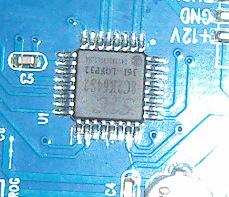
\includegraphics[width=0.8\textwidth]{pre-textuais/figuras/MicrontroladorSa202.JPG}
\caption{Microcontrolador STC8C2K64S4-36I-LQFP32 utilizado na controladora SA-202}
\label{fig:microcontrolador_sa202}
\end{figure}

\subsection{Descobrindo as Especificações do Microcontrolador}

Após identificar o modelo do microcontrolador, fui atrás do datasheet para entender suas capacidades. O STC8C2K64S4-36I-LQFP32 é baseado na arquitetura 8051 aprimorada\footnote{A arquitetura 8051 é uma das mais antigas e populares para microcontroladores de 8 bits, criada pela Intel em 1980.}, funcionando com um clock de até 36 MHz, o que é bem rápido para um microcontrolador dessa categoria. Ele possui 64KB de memória Flash para armazenar o programa e 2KB de RAM interna para processamento, além de interface de comunicação serial UART que poderia ser útil para interceptar os dados.

O chip vem em um encapsulamento LQFP32, com 32 pinos disponíveis, e opera com tensão entre 3.3V e 5.5V, o que daria flexibilidade para trabalhar com diferentes níveis lógicos. Consegui baixar o datasheet completo, mas me deparei com um problema inesperado: eram 956 páginas de documentação técnica, todas escritas em chinês. Mesmo usando tradutores online, a compreensão dos detalhes técnicos mais complexos ficou extremamente difícil.

% [INSERIR FIGURA: Diagrama de pinagem do microcontrolador]
\begin{figure}[htbp!]
\centering
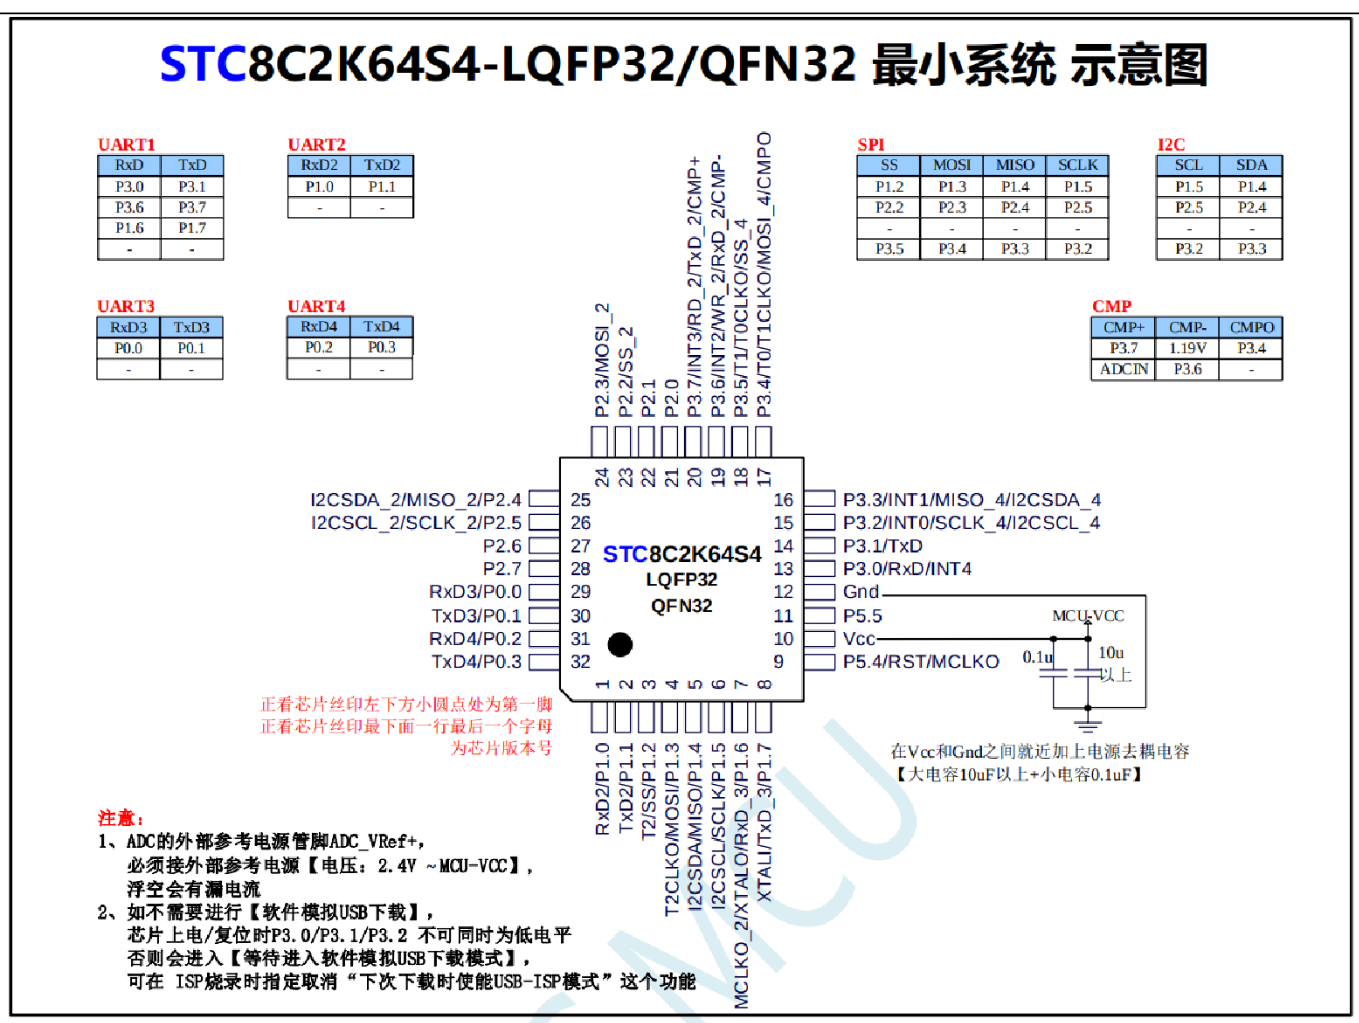
\includegraphics[width=0.9\textwidth]{pre-textuais/figuras/pinagem_stc8c2k..png}
\caption{Diagrama de pinagem do microcontrolador STC8C2K64S4-36I-LQFP32}
\label{fig:pinagem_micro}
\end{figure}

\section{Desafios Técnicos Encontrados}
\label{sec:desafios}

A tentativa de integração direta com a controladora se mostrou muito mais complexa do que eu havia imaginado inicialmente. Passei dias tentando interceptar os sinais de comunicação entre o microcontrolador e o leitor RFID. Utilizei um jumper conectado em outro microcontrolador para poder interceptar algum sinal da comunicação serial. No entanto, o protocolo utilizado era completamente proprietário e, mesmo monitorando os sinais UART, não consegui decodificar o formato dos dados transmitidos.

\subsection{Barreiras para Reprogramação}

Quando percebi que não conseguiria simplesmente interceptar os sinais, pensei em reprogramar o microcontrolador para adicionar as funcionalidades que precisava. Foi então que descobri outro obstáculo: o STC8C2K64S4-36I-LQFP32 requer um programador específico, o AI8H2K12U, para gravar novo firmware. Procurei esse equipamento em todas as lojas de eletrônica que conhecia e em diversos sites nacionais, mas simplesmente não existe disponibilidade desse programador no Brasil. Importar da China levaria meses e teria um custo elevado.

Além da questão do hardware, a barreira linguística tornou-se um problema sério. Com 956 páginas de documentação completamente em chinês, mesmo usando o Google Tradutor e outros recursos, não conseguia compreender com segurança os detalhes necessários para reprogramar o chip sem danificá-lo. Termos técnicos específicos perdiam o sentido na tradução, e eu não tinha confiança de que estava interpretando corretamente os procedimentos.

\subsection{Riscos de Modificar o Sistema Original}

Mesmo que conseguisse superar essas barreiras técnicas, precisava considerar os riscos envolvidos em modificar diretamente a controladora. A possibilidade real de danificar permanentemente a controladora durante as tentativas de reprogramação era muito preocupante, pois deixaria a porta sem nenhum sistema de controle de acesso.

Além disso, mexer no firmware original poderia criar vulnerabilidades não previstas, comprometendo todo o sistema de segurança. Qualquer erro poderia tornar o equipamento inutilizável. 

\section{Solução Proposta: Interceptação do Sinal RFID}
\label{sec:solucao-proposta}

Diante dos desafios identificados, foi desenvolvida uma solução alternativa baseada na interceptação do sinal RFID diretamente na fonte, antes do processamento pela controladora original. Esta abordagem permite a captura dos dados das tags sem interferir no funcionamento do sistema existente, garantindo assim a integridade operacional da controladora SA-202.

\subsection{Arquitetura da Solução Desenvolvida}

Foi quando tive a ideia que salvou o projeto: em vez de tentar modificar a controladora, por que não criar um sistema paralelo que funcionasse junto com ela? A solução que desenvolvi permite que ambos os sistemas operem simultaneamente sem interferência mútua. 

O coração da solução é o módulo RDM6300, um leitor RFID que comprei para fazer os testes. Esse módulo seria conectado em paralelo com a antena original, permitindo que ele lesse as mesmas tags que a controladora SA-202. Para processar os dados do RDM6300, utilizei um Arduino Uno que tinha disponível em casa. O Arduino seria responsável por receber os dados via UART, validá-los e repassá-los para o próximo componente.

Para adicionar conectividade ao sistema, integrei um módulo ESP8266\footnote{System-on-Chip (SoC) Wi-Fi desenvolvido pela Espressif Systems, amplamente utilizado em projetos IoT.}, que é basicamente um microcontrolador com Wi-Fi integrado. Esse módulo seria responsável por enviar os dados para o Firebase. Como o Arduino opera com lógica de 5V e o ESP8266 com 3.3V, precisei adicionar um conversor de nível lógico entre eles para garantir que os sinais fossem transmitidos corretamente sem danificar nenhum componente.

% [INSERIR FIGURA: Diagrama da arquitetura do sistema]
\begin{figure}[htbp!]
\centering
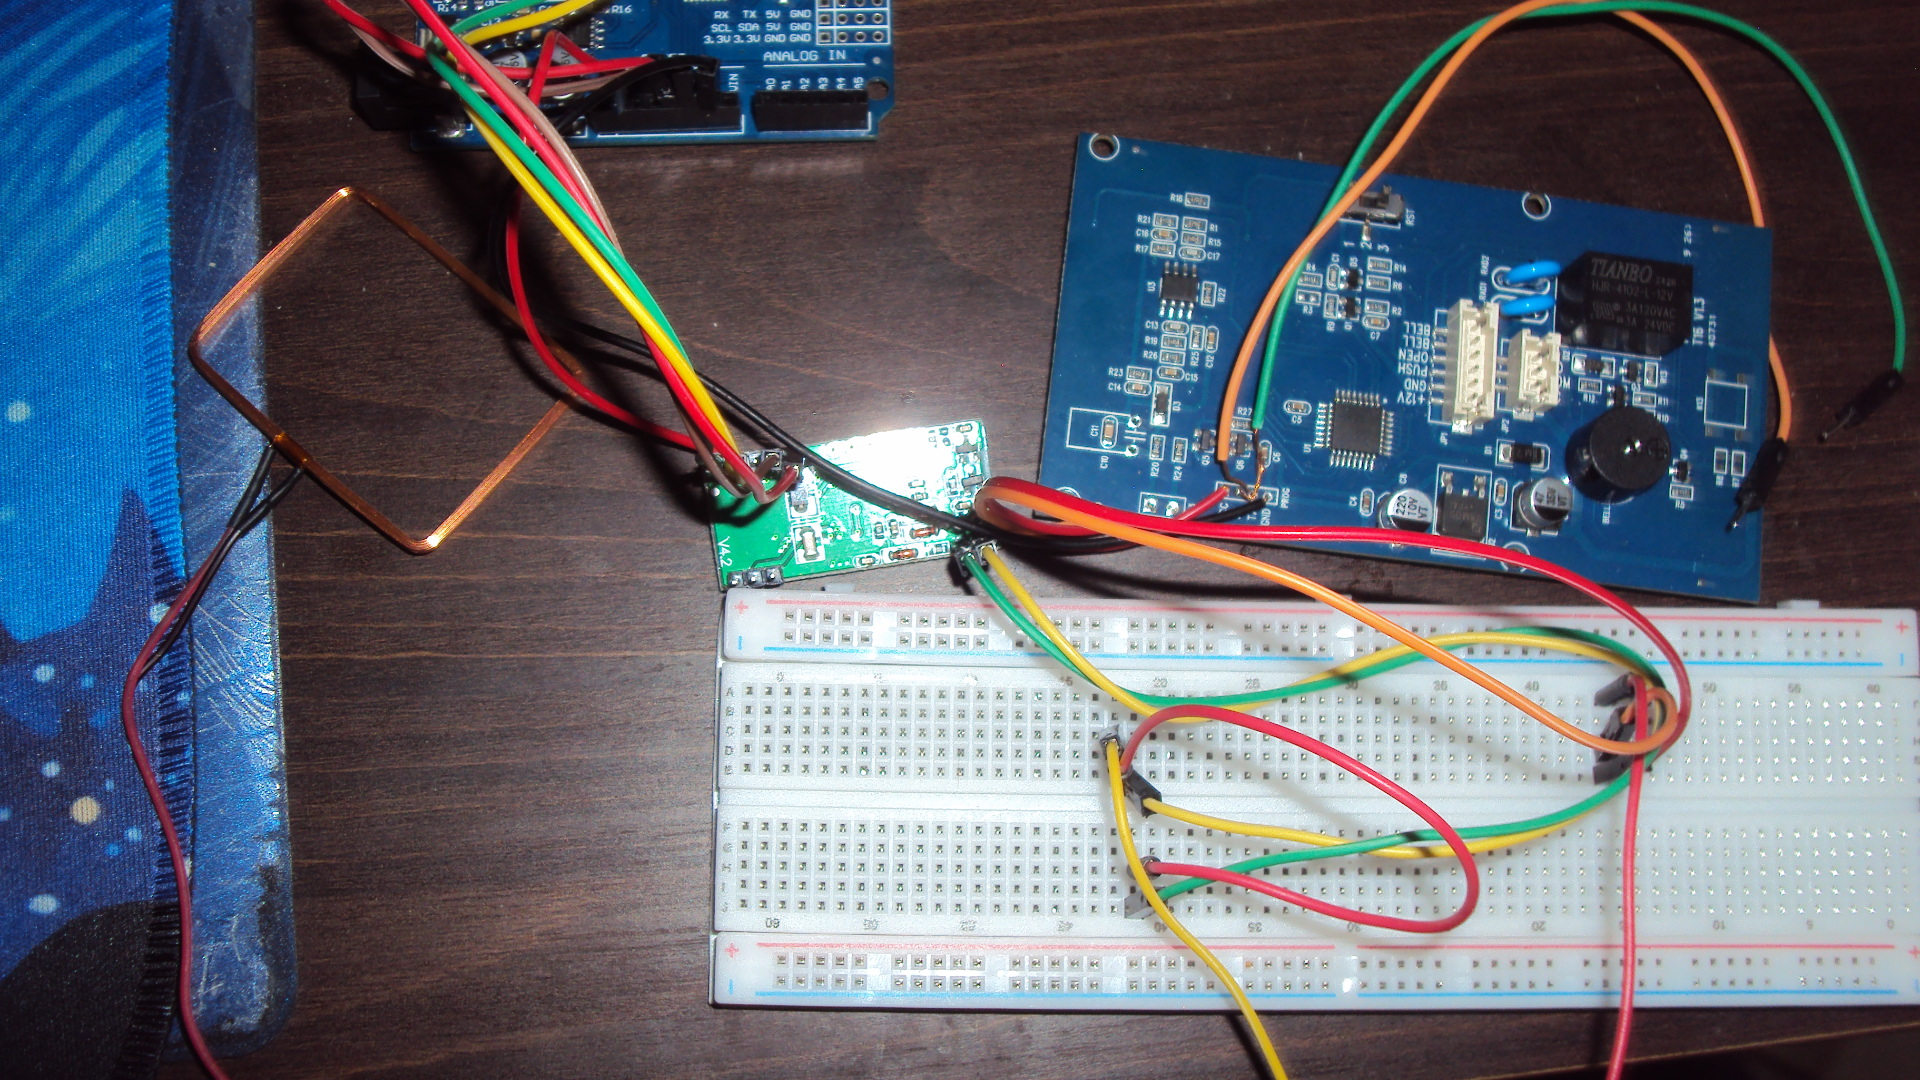
\includegraphics[width=0.8\textwidth]{pre-textuais/figuras/EsquemadeLigaçãoRDMSA202.JPG}
\caption{Arquitetura do sistema de interceptação RFID proposto}
\label{fig:arquitetura}
\end{figure}

\subsection{Escolha do Módulo RDM6300}

A escolha do RDM6300\footnote{Módulo leitor RFID de baixo custo que opera em 125 kHz, compatível com tags EM4100.} como leitor RFID não foi por acaso. Pesquisei vários módulos disponíveis no mercado e esse se destacou por várias razões. Primeiro e mais importante, ele opera exatamente na mesma frequência da controladora SA-202, 125 kHz, o que significa que poderia ler as mesmas tags sem nenhuma modificação. Além disso, sua interface de comunicação UART é extremamente simples, operando no padrão 9600 bps que qualquer microcontrolador consegue trabalhar facilmente.

Outro ponto decisivo foi a documentação. Diferente do microcontrolador chinês da controladora, o protocolo do RDM6300 está bem documentado em inglês, com exemplos claros de implementação, como detalhado na Seção \ref{sec:leitor-rdm630} do Capítulo \ref{Cap:Teoria}. E o melhor de tudo: consegui comprar o módulo no Mercado Livre por aproximadamente R\$ 45,00, tornando a solução economicamente viável.

% [INSERIR FIGURA: Módulo RDM6300]
\begin{figure}[htbp!]
\centering
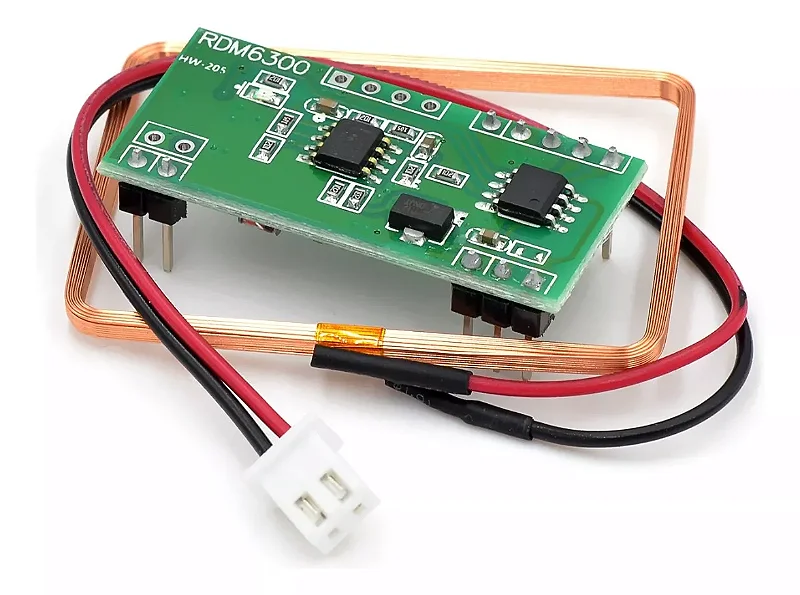
\includegraphics[width=0.6\textwidth]{pre-textuais/figuras/RDM6300PNG.png}
\caption{Módulo leitor RFID RDM6300}
\label{fig:rdm6300}
\end{figure}

\section{Implementação do Sistema de Leitura RFID}
\label{sec:implementacao-rfid}

\subsection{Entendendo o Protocolo de Comunicação}

Quando comecei a trabalhar com o RDM6300, precisei primeiro entender como ele transmite os dados das tags lidas. O módulo usa um protocolo bem estruturado via UART, enviando os dados em um formato de quadro específico que precisei decodificar no Arduino.

Cada vez que uma tag é aproximada do leitor, ele envia uma sequência de 14 bytes. O primeiro byte é sempre 0x02, que é o código ASCII para STX (Start of Text), indicando o início da transmissão. Em seguida, vêm 10 bytes de dados, sendo os 2 primeiros a versão do protocolo e os 8 seguintes o ID único da tag, codificados em ASCII hexadecimal. Depois dos dados, temos 2 bytes de checksum para verificar se a transmissão foi correta, e finalmente o byte 0x03 (ETX - End of Text) marca o fim do quadro.

\subsection{Desenvolvendo o Algoritmo de Leitura}

Para processar esses dados no Arduino, desenvolvi um algoritmo que funciona como uma máquina de estados. O programa fica constantemente monitorando a porta serial conectada ao RDM6300, esperando pelo byte de início 0x02. Quando esse byte é detectado, o algoritmo começa a armazenar os próximos bytes em um buffer.

\begin{algorithm}[H]
\caption{Algoritmo de Leitura RFID Implementado}
\label{algo:leitura-rfid}
\Inicio{
    Configura porta serial SoftwareSerial em 9600 bps\;
    Cria buffer de 14 bytes para armazenar o quadro\;
    \Enqto{sistema operando}{
        \Se{byte disponível na serial}{
            lê o byte recebido\;
            \Se{byte = 0x02 (início do quadro)}{
                reseta posição do buffer para zero\;
            }
            \SenaoSe{byte = 0x03 (fim do quadro)}{
                \Se{recebeu exatamente 14 bytes}{
                    extrai os 8 bytes do ID da tag\;
                    calcula checksum usando XOR\;
                    \Se{checksum confere com o recebido}{
                        envia ID da tag pela serial principal\;
                    }
                }
                limpa o buffer para próxima leitura\;
            }
            \Senao{
                armazena byte no buffer\;
                incrementa posição\;
            }
        }
    }
}
\end{algorithm}

O interessante desse algoritmo é que ele é robusto a falhas de comunicação. Se por algum motivo a transmissão for interrompida ou chegar dados corrompidos, o sistema simplesmente descarta o quadro incompleto quando detecta um novo byte de início, evitando travamentos ou leituras incorretas.

\subsection{Implementando a Validação do Checksum}

Uma parte crucial do sistema é a validação do checksum, que garante que os dados recebidos estão corretos. Descobri que o RDM6300 calcula esse checksum fazendo uma operação XOR entre todos os pares de bytes dos dados. No início, tive dificuldade para entender exatamente como funcionava, mas depois de analisar vários exemplos de transmissão, consegui implementar a validação corretamente.

O processo começa extraindo os 10 bytes de dados do quadro recebido. Como esses bytes estão em formato ASCII representando valores hexadecimais, preciso primeiro convertê-los. Por exemplo, se recebo os caracteres '4' e 'A', preciso converter para o valor hexadecimal 0x4A. Depois, aplico a operação XOR sequencialmente em todos os pares de bytes. O resultado dessa operação deve ser igual ao checksum que vem nos dois bytes antes do fim do quadro. Se não conferir, significa que houve algum erro na transmissão e o quadro é descartado.

\subsection{Montando as Conexões do Hardware}

A montagem física do sistema foi relativamente simples, mas exigiu cuidado para não danificar os componentes. Conectei o pino TX do RDM6300 ao pino 6 do Arduino, configurado como RX através da biblioteca SoftwareSerial. Essa biblioteca permite criar uma porta serial virtual em qualquer pino digital do Arduino, deixando a porta serial principal livre para debug e comunicação com o ESP8266.

A alimentação do módulo foi conectada diretamente aos 5V e GND do Arduino, já que ambos operam na mesma tensão. A parte mais delicada foi conectar a antena do RDM6300 em paralelo com a antena original da controladora SA-202. Tive que soldar cuidadosamente fios extras nos pontos de conexão da antena original, garantindo que a impedância do sistema não fosse significativamente alterada, o que poderia reduzir o alcance de leitura.

Por fim, este trabalho serve como um exemplo prático de como enfrentar limitações técnicas com criatividade e persistência. O custo total dos componentes utilizados ficou aproximadamente em: Arduino Uno R3 (R\$ 85,00), ESP8266 NodeMCU (R\$ 35,00), módulo RDM6300 com antena (R\$ 45,00), protoboard e jumpers (R\$ 25,00), resistores e componentes auxiliares (R\$ 15,00), fonte de alimentação 5V (R\$ 25,00), totalizando cerca de R\$ 230,00. Esse valor representa uma fração do que custaria substituir toda a controladora por um modelo com conectividade nativa, que pode ultrapassar R\$ 1.500,00. Mais importante ainda, a experiência adquirida e o conhecimento compartilhado podem ajudar outros desenvolvedores a superar desafios similares em seus próprios projetos.

% [INSERIR FIGURA: Esquema de conexões RDM6300-Arduino]
\begin{figure}[htbp!]
\centering
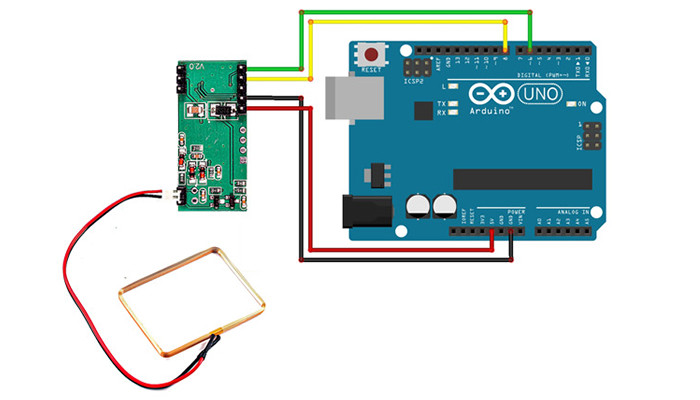
\includegraphics[width=0.8\textwidth]{pre-textuais/figuras/RdmcomArduino.png}
\caption{Esquema de conexões entre RDM6300 e Arduino Uno}
\label{fig:conexoes_arduino}
\end{figure}

\section{Integração com ESP8266 e Firebase}
\label{sec:integracao-firebase}

\subsection{Estabelecendo a Comunicação Arduino-ESP8266}

Com o sistema de leitura RFID funcionando no Arduino, o próximo desafio era enviar esses dados para a nuvem. Para isso, precisava conectar o Arduino ao ESP8266, mas havia um problema técnico importante: o Arduino opera com lógica de 5V enquanto o ESP8266 trabalha com 3.3V. Conectar diretamente poderia queimar o ESP8266, então utilizei um conversor de nível lógico bidirecional que comprei por menos de R\$ 10,00.

A comunicação entre os dois microcontroladores foi estabelecida via serial. Configurei o Arduino para enviar os IDs das tags lidas através de sua porta serial principal (pinos 0 e 1) a 115200 bps, uma taxa bem mais alta que a usada com o RDM6300 para garantir que os dados fossem transmitidos rapidamente. No ESP8266, configurei a mesma taxa para receber esses dados e processá-los.

% [INSERIR FIGURA: Esquema de ligação com conversor de nível]
\begin{figure}[htbp!]
\centering
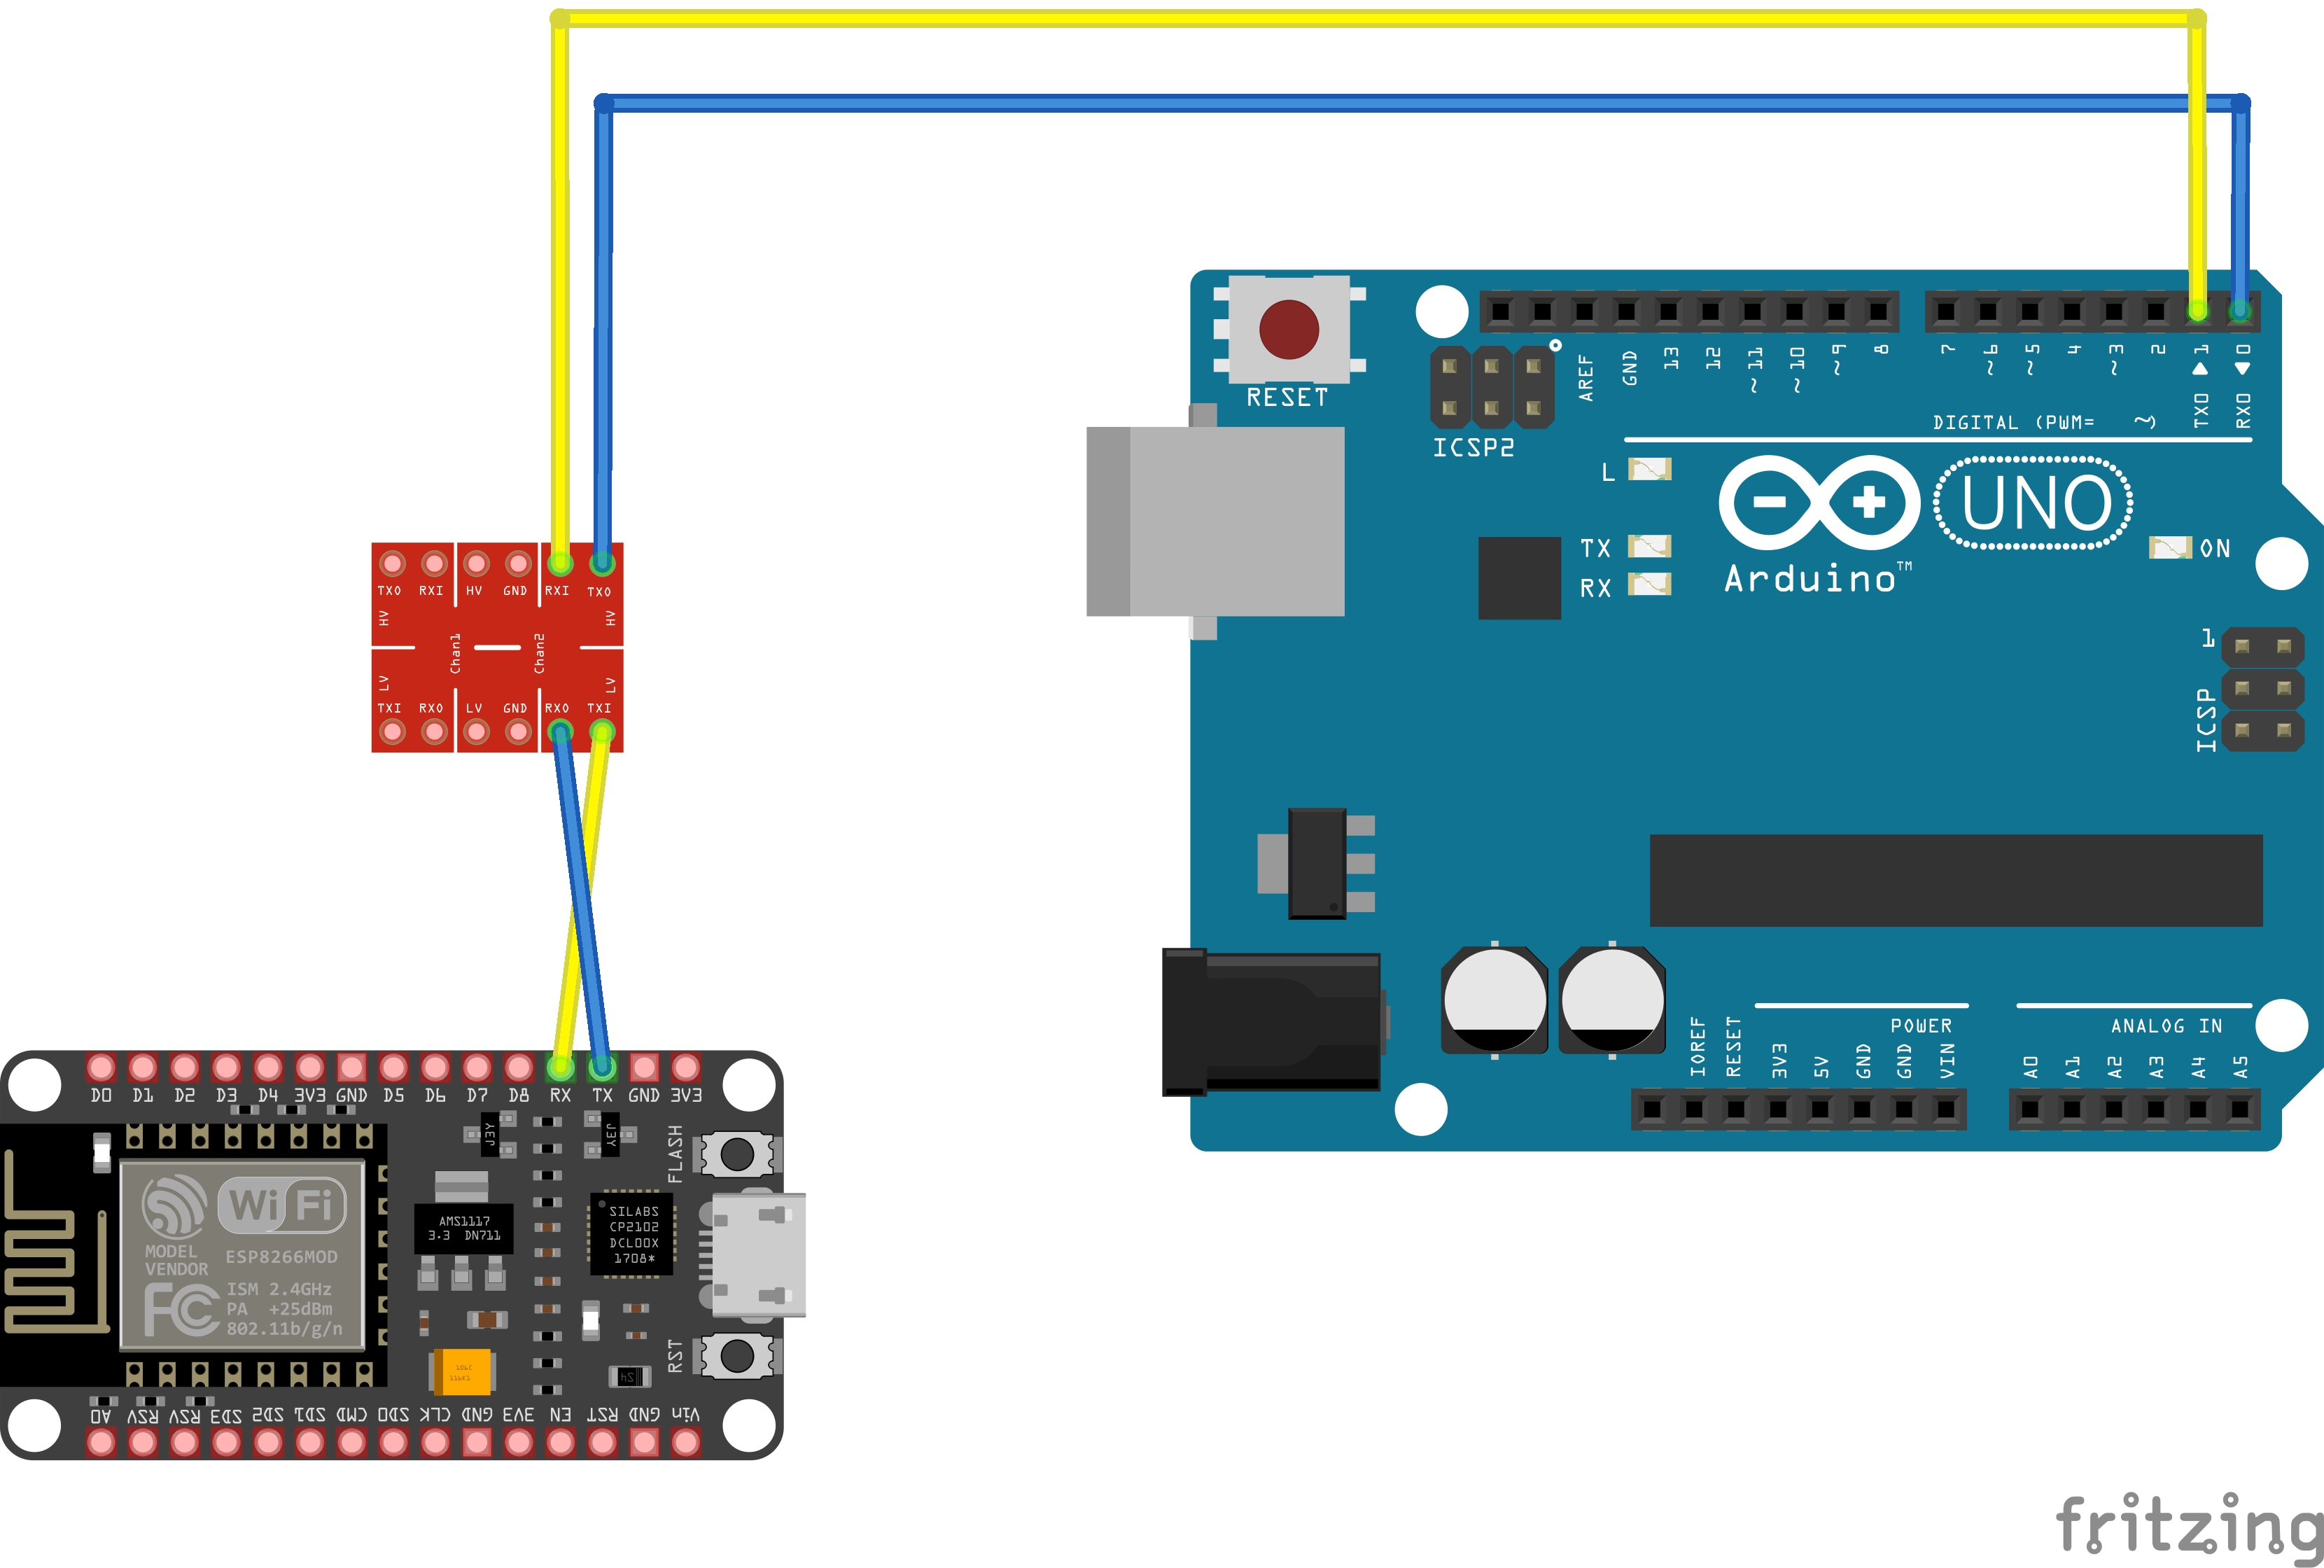
\includegraphics[width=0.8\textwidth]{pre-textuais/figuras/EsquemaArduinoESp.jpg}
\caption{Esquema de ligação com conversor de nível lógico}
\label{fig:conversor_nivel}
\end{figure}

\subsection{Implementando a Comunicação com o Firebase}

A parte mais desafiadora do projeto foi estabelecer a comunicação segura com o Firebase. Optei por usar a API REST do Firebase Realtime Database porque ela permite enviar dados via HTTPS usando requisições POST simples, sem necessidade de bibliotecas complexas que consumiriam muita memória do ESP8266.

O processo que implementei começa quando o ESP8266 recebe um ID de tag do Arduino pela serial. Primeiro, faço uma validação para garantir que o formato está correto - deve ser uma string hexadecimal de 8 caracteres. Se houver espaços, dois pontos ou hífens (comuns em diferentes formatos de representação), removo eles e converto tudo para maiúsculas para manter um padrão.

Depois da validação, construo um objeto JSON contendo o ID da tag, um timestamp baseado no millis() do ESP8266 (já que sincronização NTP seria complexidade adicional desnecessária), e um identificador do dispositivo baseado no chip ID do ESP8266. Esse JSON é então enviado via POST para o endpoint do Firebase que configurei.

\subsection{Configurando o ESP8266 para Operação}

Configurar o ESP8266 foi surpreendentemente tranquilo graças à excelente documentação da comunidade Arduino. Programei o módulo para operar em modo estação (STA), que significa que ele se conecta a uma rede Wi-Fi existente como qualquer dispositivo comum, em vez de criar seu próprio ponto de acesso.

No código, defini as credenciais da minha rede Wi-Fi doméstica (SSID e senha) e configurei o módulo para se reconectar automaticamente caso a conexão caia. A rede usa WPA2, o protocolo de segurança padrão atualmente, e o ESP8266 não teve problemas para se autenticar. A taxa de comunicação serial com o Arduino foi configurada em 115200 bps, garantindo transferência rápida dos dados.

Para a comunicação com o Firebase, utilizei a biblioteca ESP8266HTTPClient com WiFiClientSecureBearSSL para estabelecer conexões HTTPS seguras. Embora o ideal seria validar o certificado SSL do servidor, optei por usar setInsecure() durante o desenvolvimento para simplificar. Em um ambiente de produção, seria importante implementar a validação completa do certificado.

\subsection{Organizando os Dados no Firebase}

No Firebase, estruturei os dados de forma simples mas eficiente. Criei um nó chamado "reads" onde cada leitura de tag é armazenada com uma chave única gerada automaticamente pelo Firebase quando uso o método POST. Essa abordagem garante que nunca haverá conflitos de dados, mesmo com múltiplas leituras simultâneas.

Cada registro armazena o ID da tag em formato hexadecimal padronizado (8 caracteres maiúsculos), um timestamp indicando quando a leitura ocorreu, e um identificador do dispositivo que fez a leitura. Esse identificador é importante porque, no futuro, posso ter múltiplos pontos de acesso enviando dados para o mesmo banco de dados. Usei o chip ID do ESP8266, que é único para cada dispositivo, prefixado com "ESP8266-" para facilitar a identificação.

\begin{verbatim}
{
  "reads": {
    "-NxYz123abc": {
      "tag": "1A2B3C4D",
      "timestamp": 1234567890,
      "device": "ESP8266-A1B2C3D4",
      "status": "authorized"
    }
  }
}
\end{verbatim}

Inicialmente pensei em adicionar mais campos, como nome do usuário ou tipo de acesso, mas decidi manter simples. Esses dados adicionais podem ser cruzados posteriormente com outro banco de dados que mantenha o cadastro de usuários e suas respectivas tags.

\subsection{Algoritmo de Transmissão para Firebase}

O algoritmo de transmissão implementado no ESP8266 gerencia o envio dos dados para o Firebase:

\begin{algorithm}[H]
\caption{Algoritmo de Transmissão Firebase}
\label{algo:transmissao-firebase}
\Inicio{
    Conecta à rede Wi-Fi\;
    Inicializa cliente HTTPS\;
    \Enqto{sistema ativo}{
        \Se{dados recebidos via serial}{
            Valida formato hexadecimal\;
            \Se{formato válido}{
                Constrói payload JSON\;
                Adiciona timestamp\;
                Adiciona ID do dispositivo\;
                Envia requisição POST\;
                \Se{resposta HTTP 2xx}{
                    Registra sucesso\;
                }
                \Senao{
                    Registra erro\;
                    Tenta reenvio\;
                }
            }
        }
    }
}
\end{algorithm}

\subsection{Tratamento de Dados Hexadecimais}

Um detalhe importante que precisei implementar foi o tratamento adequado dos dados hexadecimais. Quando recebo uma tag do Arduino, ela pode vir em diferentes formatos dependendo de como foi lida ou processada. Às vezes vem com espaços entre os bytes, outras vezes com dois pontos ou hífens como separadores. Para garantir consistência no banco de dados, criei uma função de normalização que remove todos esses caracteres separadores e converte tudo para maiúsculas.

Além da normalização, é crucial validar que todos os caracteres são hexadecimais válidos (0-9 e A-F). Já tive problemas onde ruído na comunicação serial gerava caracteres inválidos, e sem essa validação, dados corrompidos seriam enviados ao Firebase. A verificação final confirma que o ID tem exatamente 8 caracteres, que é o tamanho padrão das tags EM4100 de 125 kHz.

\section{Interface Web de Monitoramento}
\label{sec:interface-web}

Uma funcionalidade adicional que implementei foi uma interface web simples diretamente no ESP8266. Isso me permite monitorar e testar o sistema sem precisar conectar cabos ou usar o monitor serial. O ESP8266 tem capacidade de processar requisições HTTP enquanto mantém a comunicação com o Firebase, então aproveitei isso para criar alguns endpoints úteis.

\subsection{Criando os Endpoints HTTP}

O servidor web que implementei é bem simples mas funcional. A página principal, acessível pela raiz (/), mostra instruções básicas de uso e confirma que o sistema está operacional. Criei também um endpoint especial /setTag que aceita um parâmetro "code" na URL. Isso me permite testar o envio de tags para o Firebase sem precisar de uma tag física - basta acessar algo como "http://192.168.1.100/setTag?code=1A2B3C4D" no navegador. Tem também um endpoint /status que retorna o estado atual do sistema em formato JSON, útil para integrações futuras.

\subsection{Recursos de Monitoramento}

Através dessa interface web, consigo monitorar vários aspectos do sistema em tempo real. Posso ver se a conexão Wi-Fi está estável, verificar se a comunicação com o Firebase está funcionando, visualizar as últimas tags que foram lidas e até manter um contador de quantos acessos foram registrados desde a última reinicialização. Quando algo dá errado, o log de erros me ajuda a identificar rapidamente se o problema é na rede, no Firebase ou na leitura das tags.

\section{Integração Paralela com Controladora Original}
\label{sec:integracao-paralela}

\subsection{Fazendo a Conexão Paralela}

O momento mais tenso do projeto foi quando conectei meu sistema em paralelo com a controladora original. Precisava garantir que ambos funcionassem simultaneamente sem interferência. A solução foi conectar a antena do RDM6300 diretamente nos mesmos pontos da antena da SA-202, criando essencialmente duas "orelhas" escutando o mesmo sinal.

Essa configuração acabou sendo perfeita porque mantém a funcionalidade original intacta - se meu sistema falhar ou for desligado, a porta continua funcionando normalmente. Além disso, tenho uma captura redundante dos dados, o que é ótimo para backup. Cada sistema opera de forma completamente independente, e posso desativar o meu para manutenção sem afetar o controle de acesso.

% [INSERIR FIGURA: Esquema de conexão paralela das antenas]
\begin{figure}[htbp!]
\centering
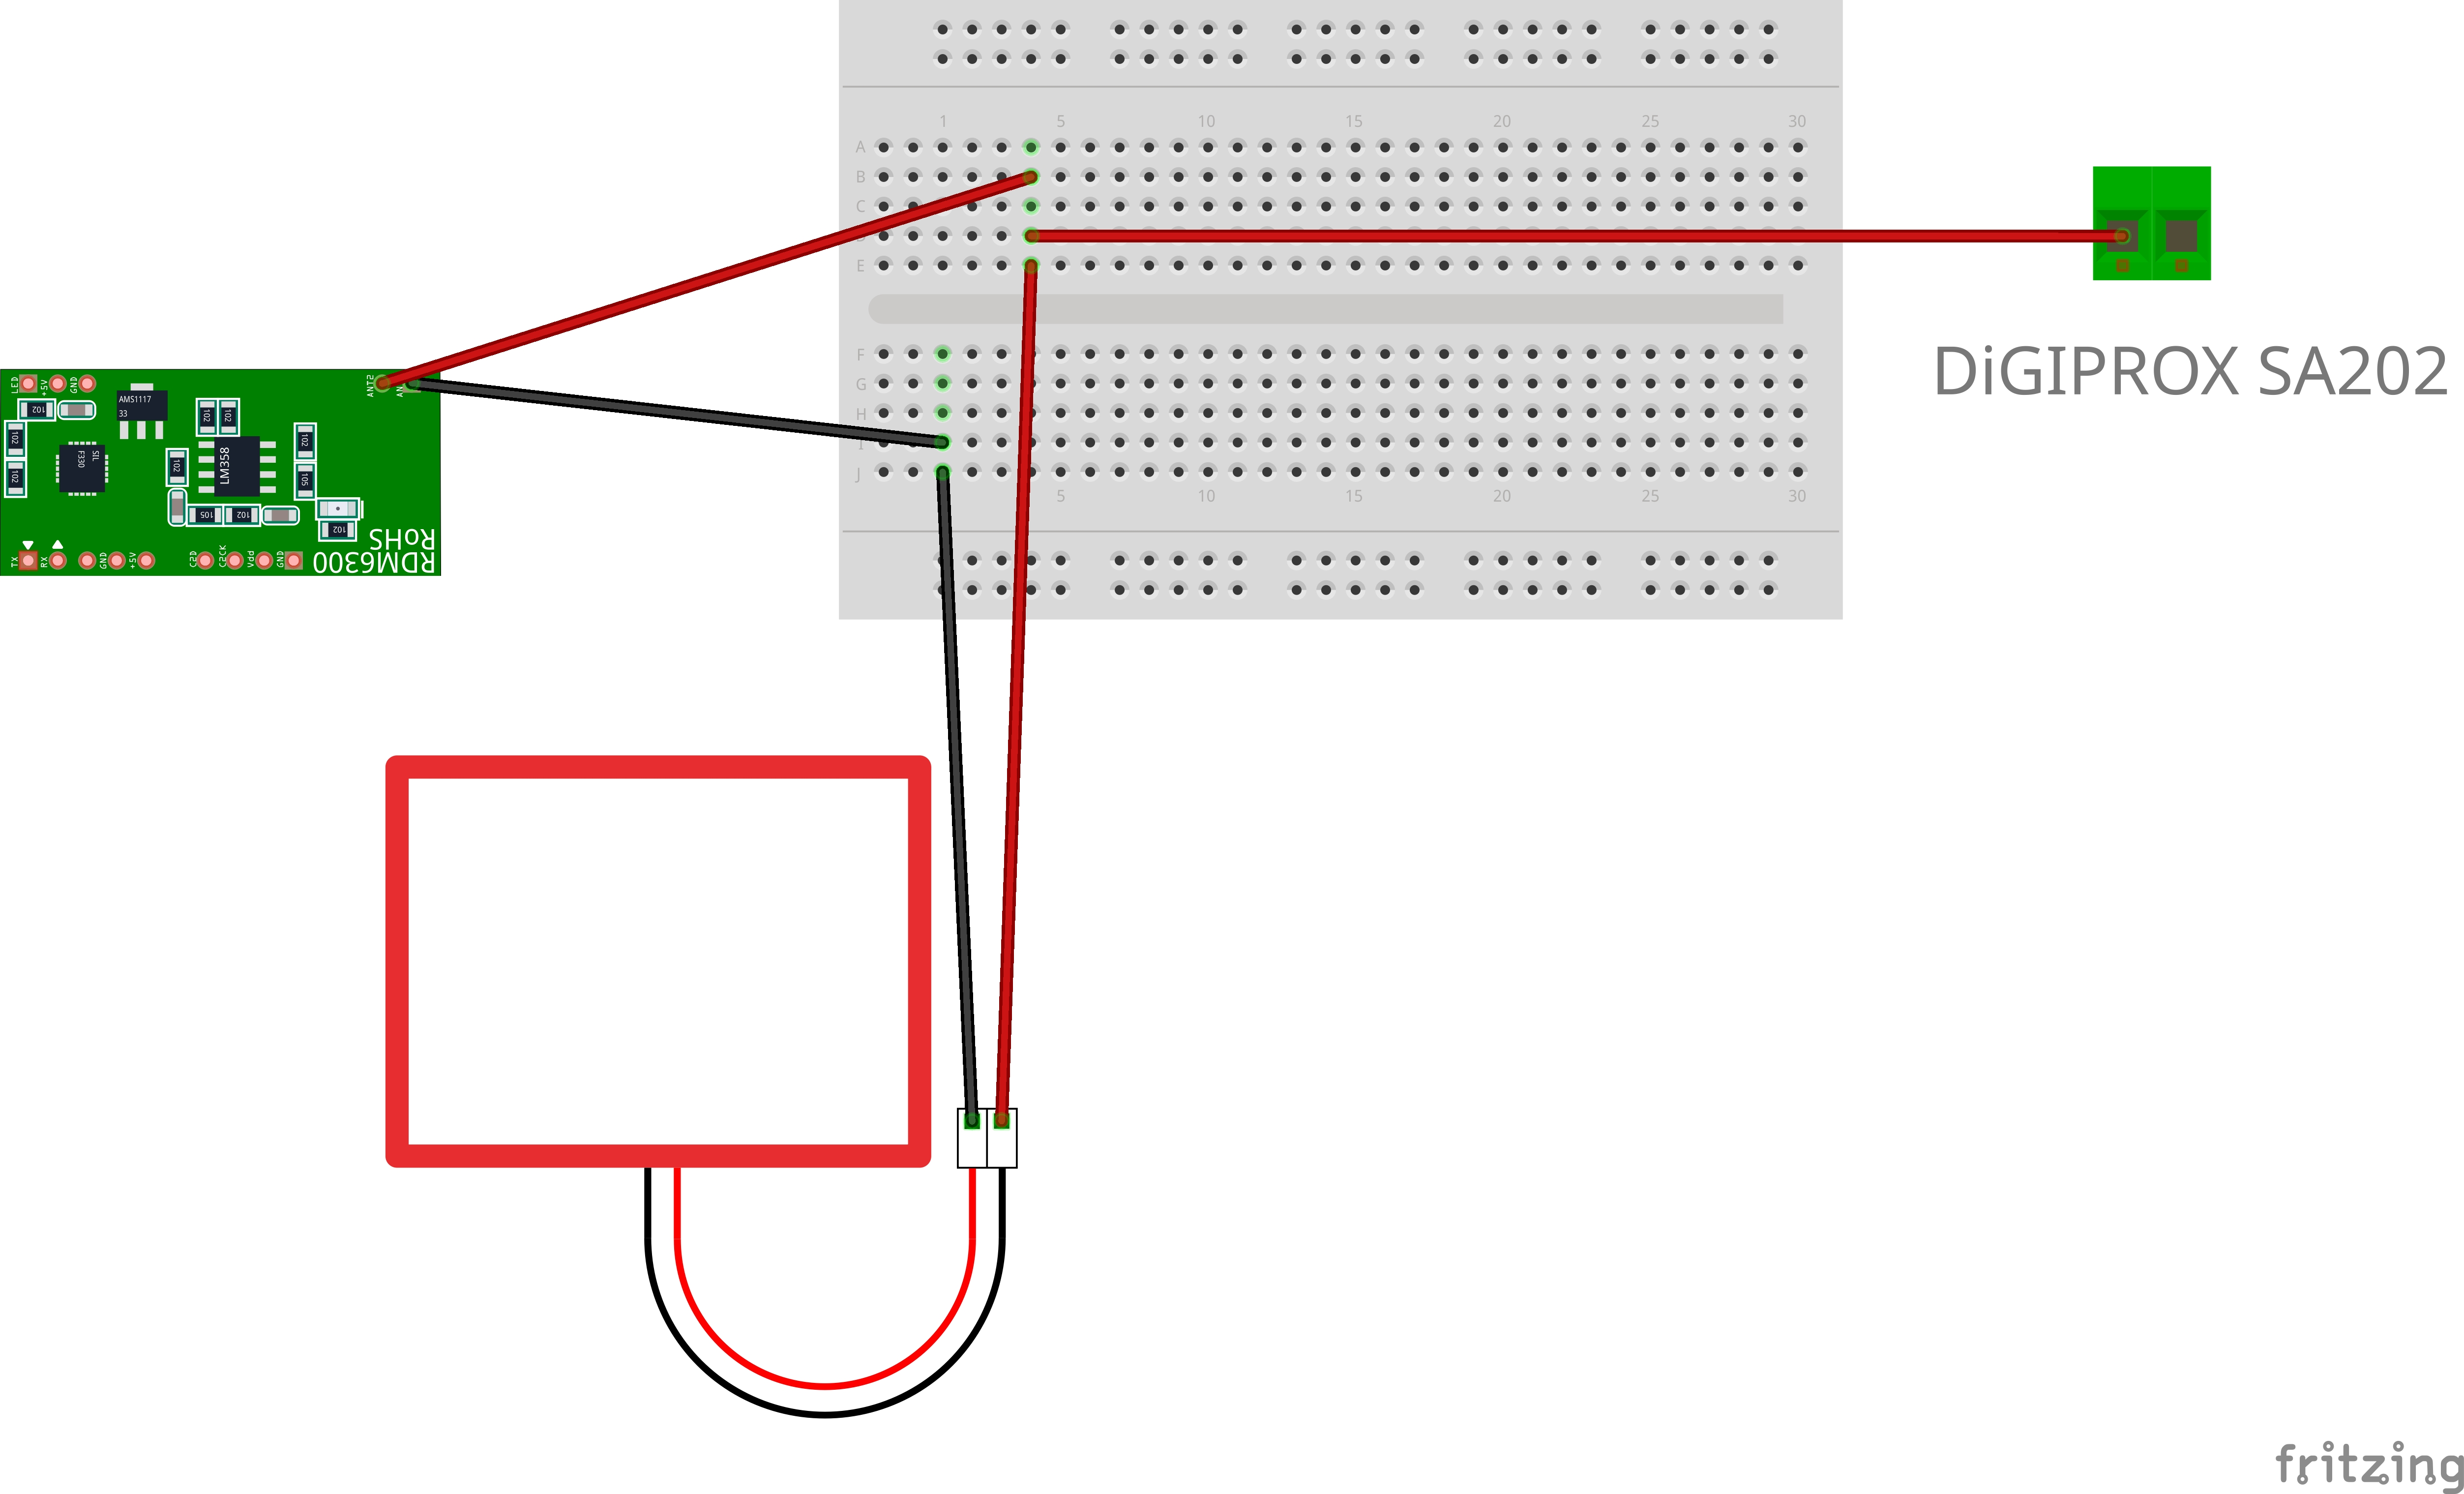
\includegraphics[width=0.8\textwidth]{pre-textuais/figuras/esquemaEmparalelo.jpg}
\caption{Esquema de conexão paralela das antenas RFID}
\label{fig:conexao_paralela}
\end{figure}

\subsection{Garantindo a Sincronização dos Dados}

Para garantir que nenhum dado seja perdido, implementei vários mecanismos de proteção. O mais importante é o buffer local no ESP8266 que armazena temporariamente as leituras quando a conexão com a internet cai. Configurei um sistema de retry automático que tenta reenviar os dados não confirmados a cada 30 segundos.

Cada leitura recebe um timestamp local baseado no millis() do ESP8266, garantindo que mesmo sem sincronização NTP eu tenha uma referência temporal relativa. Para evitar duplicatas no banco de dados, cada registro inclui um identificador único composto pelo chip ID do ESP8266 e o timestamp, tornando praticamente impossível ter colisões.

\section{Considerações Finais}
\label{sec:consideracoes-implementacao}

\subsection{Principais Desafios Superados}

Ao longo do desenvolvimento, enfrentei e superei vários desafios técnicos que pareciam intransponíveis no início. O primeiro foi entender e decodificar o protocolo do RDM6300, que embora documentado, tem suas peculiaridades que só descobri na prática. A sincronização entre o Arduino e o ESP8266 operando em velocidades diferentes também exigiu ajustes finos para evitar perda de dados.

Implementar comunicação segura com o Firebase foi outro desafio interessante. Tive que equilibrar segurança com as limitações de memória do ESP8266, optando por uma solução pragmática que funciona bem para o escopo do projeto. O tratamento de falhas de conectividade exigiu criatividade para implementar um sistema de buffer e retry que não consumisse toda a memória disponível. E otimizar o código para caber nos recursos limitados dos microcontroladores foi um exercício constante de refatoração e otimização.

\subsection{Limitações do Sistema}

É importante reconhecer as limitações do sistema implementado. A dependência de uma conexão Wi-Fi estável é provavelmente a maior delas - sem internet, os dados não são enviados para o Firebase, embora o sistema de buffer ajude a mitigar perdas temporárias. O alcance de leitura de 5 centímetros é uma característica da tecnologia de 125 kHz e pode ser inconveniente em algumas situações.

A capacidade do buffer local é limitada a cerca de 100 registros devido às restrições de memória do ESP8266. Em caso de perda prolongada de conectividade, registros mais antigos seriam descartados. Além disso, o sistema precisa de alimentação constante, não sendo viável para operação com bateria devido ao consumo do Wi-Fi.

\subsection{Sugestões para Trabalhos Futuros}

Existem várias melhorias que poderiam ser implementadas em versões futuras do projeto. A adição de um cartão SD permitiria armazenamento local praticamente ilimitado, garantindo que nenhum registro seja perdido mesmo com quedas prolongadas de internet. Um display LCD tornaria o sistema mais amigável, mostrando informações de status e confirmações visuais das leituras.

O desenvolvimento de um aplicativo móvel dedicado elevaria o projeto a outro nível, permitindo gerenciamento completo do sistema, notificações push e visualização de relatórios detalhados. Implementar autenticação de dois fatores aumentaria significativamente a segurança, enquanto a integração com sistemas de gestão empresarial existentes ampliaria as possibilidades de uso em ambientes corporativos.

Este capítulo detalhou todo o processo de implementação do sistema, desde os desafios iniciais com a controladora proprietária até a solução final funcionando em paralelo. A abordagem adotada, utilizando componentes de baixo custo e código aberto, provou que é possível modernizar sistemas legados sem grandes investimentos. Os conhecimentos teóricos apresentados nos Capítulos \ref{Cap:Teoria} e os requisitos definidos no Capítulo \ref{Cap:Problema} foram fundamentais para guiar as decisões técnicas e garantir o sucesso do projeto.
